\documentclass{ctexart}
    \usepackage{mathrsfs}
    \usepackage{multirow}
    \usepackage{graphicx}
    \usepackage{array}
    \usepackage{makecell}
    \usepackage{amsmath}
    \usepackage{booktabs}
    \usepackage{float}
    \usepackage{diagbox}
    \newcommand\mgape[1]{\gape{$\vcenter{\hbox{#1}}$}}
    \newcommand\Ronum[1]{\uppercase\expandafter{\romannumeral #1\relax}}
    \newcommand\ronum[1]{\romannumeral #1\relax}
    \author{钱思天\ 1600011388 No.8}
    \title{实验十七\ RLC电路的谐振现象 \ 实验报告}
    \begin{document}
      \maketitle
      \section{实验数据与处理}
      根据实验的初始设定,以及各仪器的误差计算公式如:$$\mbox{电容箱允差:}\pm0.65\%(0.01\mu F\mbox{档})$$
          $$\mbox{标准电感允差:}\pm0.1\%$$
          $$e_R=0.1\Omega$$      
      
         得关于已知物理量,其值如下表:
        % Table generated by Excel2LaTeX from sheet 'Sheet1'
\begin{table}[H]
  \centering
  \caption{已知物理量表}
    \begin{tabular}{|c|c|c|c|}\hline
    已知物理量 & 电容$C$ & 电感$L$ & 电阻$R$ \\\hline
    值     & $0.05\mu F$ & $0.1H$ & $100\Omega$ \\\hline
    允差    & $3.25\times 10^{-4}\mu F$ & $1\times 10^{-4}H$ & $0.1\Omega $ \\\hline
    \end{tabular}%
  \label{tab:addlabel}%
\end{table}%
      \subsection{谐振频率的测量}
      \subsubsection{实验数据列表}
        
经利萨茹图形完成谐振频率的确定,并通过数字万用表完成各待测电压值的测量,并根据各仪器允差的确定方法:
$$\mbox{谐振频率允差:}\pm0.001kHz(\mbox{小一个数量级改变无明显效应})$$

$$\mbox{万用表交流电压档允差:}\pm(0.2\%+\mbox{十个字})$$
得关于测量物理量有下表:
% Table generated by Excel2LaTeX from sheet 'Sheet1'
\begin{table}[H]
  \centering
  \caption{本实验测量物理量表}
    \begin{tabular}{|c|c|c|c|c|}\hline
    测量物理量 & 谐振频率$f_0$ & 电路总电压$U$ & 电阻电压$U_R$ & 电容电压$U_C$ \\\hline
    值     & $2.2600kHz$ & $0.7001V$` & $0.5256V$ & $7.313V$ \\\hline
    允差    & $0.001kHz$ & $2.4\times 10^{-3}V$ & $2.1\times10^{-3}$ & $1.5\times10^{-2}V$ \\\hline
    \end{tabular}%
  \label{tab:addlabel}%
\end{table}%
\subsubsection{计算$Q$值}
根据实测数据,由公式可计算$Q_1$得:
$$Q_1=\frac{1}{\omega_0R'C}=\frac{U_R}{2\pi f_0 R C U}=10.573$$

下计算不确定度,考虑:
$$\frac{\sigma_{Q_1}}{Q_1}=\sqrt{(\frac{\sigma_R}{R})^2+(\frac{\sigma_C}{C})^2+(\frac{\sigma_U}{U})^2+(\frac{\sigma_{U_R}}{U_R})^2++(\frac{\sigma_{f_0}}{f_0})^2}$$

又:
$$\sigma_R=\frac{e_R}{\sqrt{3}}\Rightarrow \frac{\sigma_R}{R}=6\times 10^{-4}$$
$$\sigma_C=\frac{e_C}{\sqrt{3}}=\frac{0.65\%C}{sqrt{3}}\Rightarrow\frac{\sigma_C}{C}=4\times10^{-3}$$
$$\sigma_U=\frac{e_U}{sqrt{3}}\Rightarrow\frac{\sigma_U}{U}=2\times10^{-3}$$
$$\sigma_{U_R}=\frac{e_{U_R}}{\sqrt{3}}\Rightarrow\frac{\sigma_{U_R}}{U_R}=2\times10^{-3}$$
$$\sigma_{f_0}=\frac{e_{f_0}}{\sqrt{3}}\Rightarrow\frac{\sigma_{f_0}}{f_0}=3\times10^{-4}$$

得:$$\sigma_{Q_1}=Q_1\cdot\sqrt{(\frac{\sigma_R}{R})^2+(\frac{\sigma_C}{C})^2+(\frac{\sigma_U}{U})^2+(\frac{\sigma_{U_R}}{U_R})^2++(\frac{\sigma_{f_0}}{f_0})^2}=0.05$$
$$Q_1\pm\sigma_{Q_1}=10.57\pm0.05$$

同时可根据实测数据及公式计算$Q_2$得:
$$Q_2=\frac{U_C}{U}=10.445$$

下计算不确定度,考虑:
$$\frac{\sigma_{Q_2}}{Q_2}=\sqrt{(\frac{\sigma_U}{U})^2+(\frac{\sigma_{U_C}}{U_C})^2}$$

又:
$$\sigma_{U_C}=\frac{e_{U_C}}{\sqrt{3}}\Rightarrow\frac{\sigma_{U_C}}{U_C}=1\times10^{-3}$$
$$\sigma_U=\frac{e_U}{sqrt{3}}\Rightarrow\frac{\sigma_U}{U}=2\times10^{-3}$$

得:
$$\sigma_{Q_2}=Q_2\cdot\sqrt{(\frac{\sigma_U}{U})^2+(\frac{\sigma_{U_C}}{U_C})^2}=0.02$$
$$Q_2\pm\sigma_{Q_2}=10.45\pm0.02$$
\subsection{相频特性曲线的测定}
调节信号发生器产生的电压频率,借助示波器观察,并根据公式$\Delta \phi = \Delta t \times f \times 360^\circ$,得如下数据表:
% Table generated by Excel2LaTeX from sheet 'Sheet1'
\begin{table}[H]
  \centering
  \caption{相频关系实测数据表}
    \begin{tabular}{|c|c|c|c|c|c|c|c|}\hline
    $f/kHz$ & 1.754 & 1.966 & 2.089 & 2.159 & 2.201 & 2.232 & 2.260 \\\hline
    $\phi/^\circ$ & -79.6 & -71.8 & -58.3 & -43.9 & -29.3 & -16.1 & 0.0 \\\hline
    $f/kHz$ & 2.287 & 2.320 & 2.365 & 2.447 & 2.598 & 2.918 & - \\\hline
    $\phi/^\circ$ & 13.2  & 29.6  & 45.5  & 59.9  & 71.1  & 79.3  &-  \\\hline
    \end{tabular}%
  \label{tab:addlabel}%
\end{table}%
根据实测数据,得图像如下:
\begin{figure}[H]
  \centering
  \caption{相频特性曲线图}
  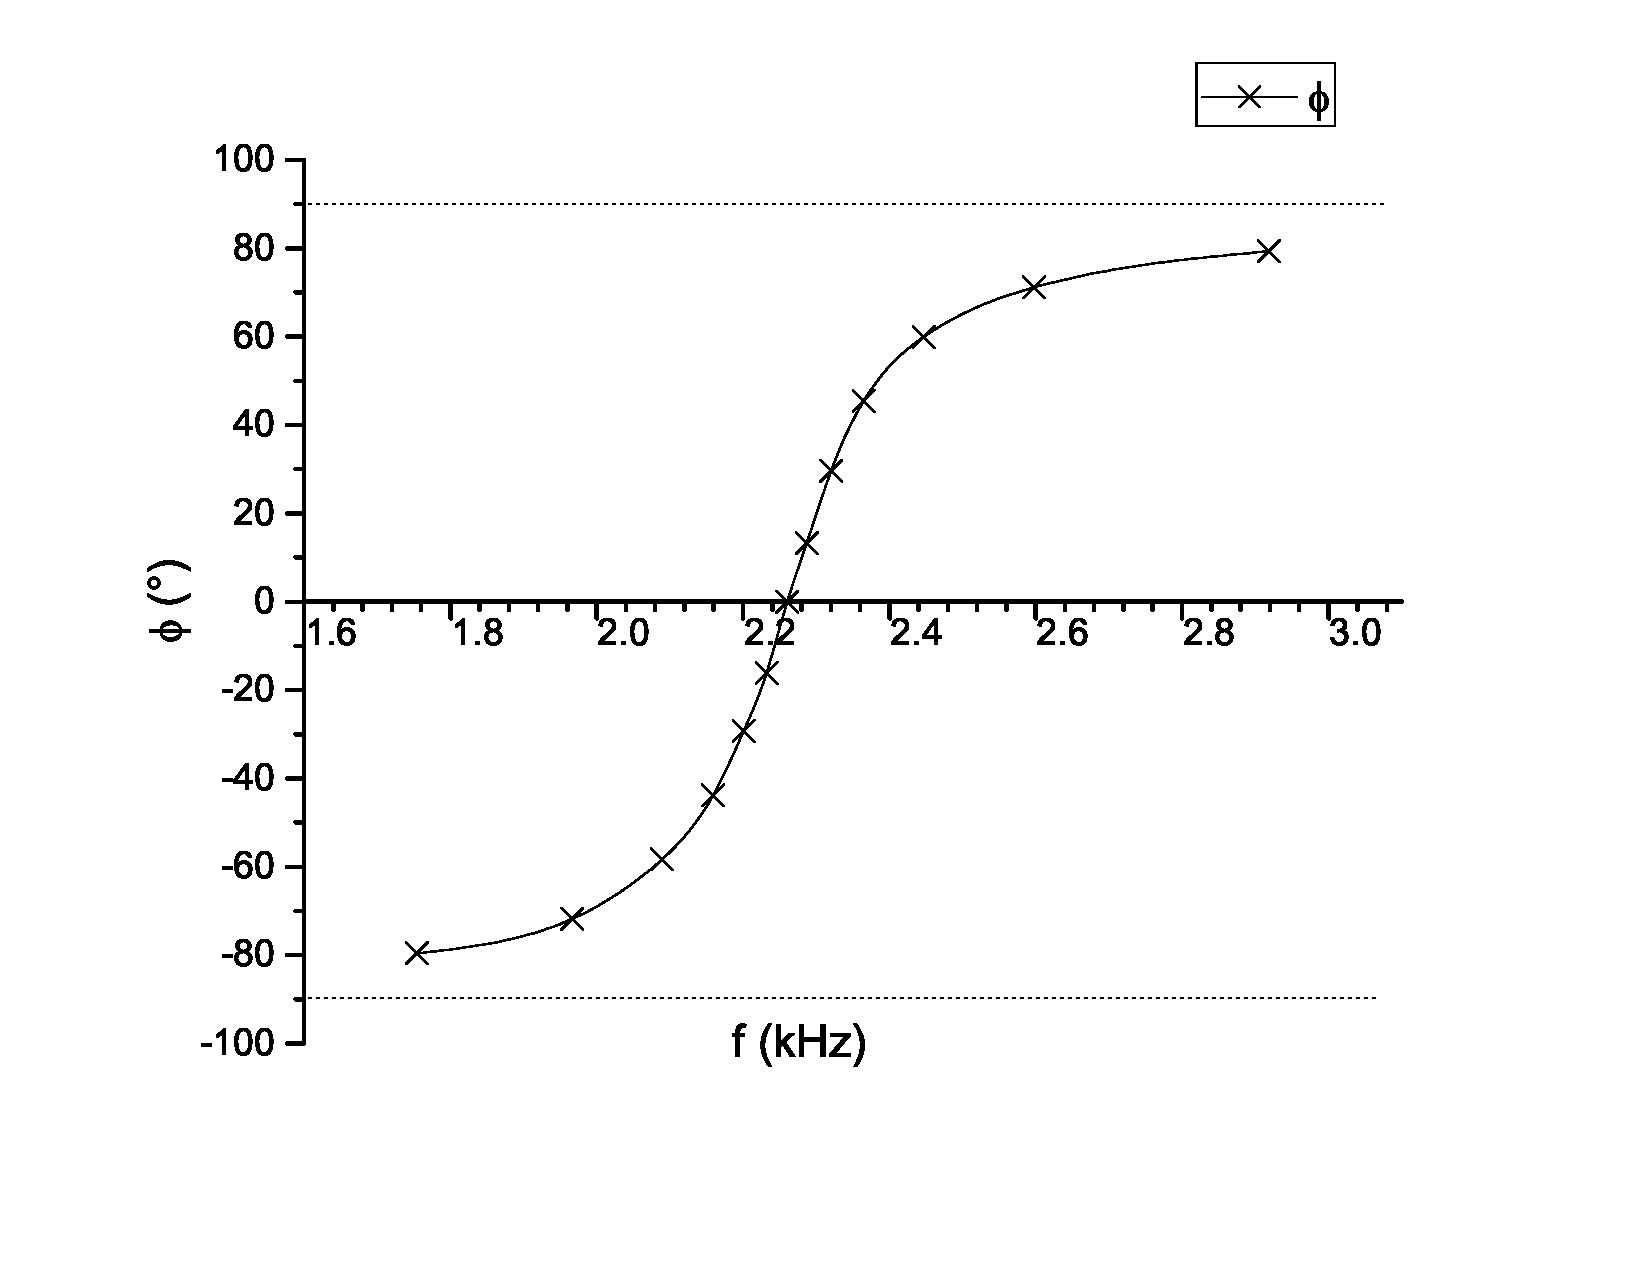
\includegraphics[width=1.0\textwidth]{1}
  \label{fig:digit}
\end{figure}
\subsection{幅频特性曲线的测定}
调节信号发生器产生的电压频率,借助数字万用表监控,保持$U=1V$,并借助公式$i=\frac{U_R}{R}$得如下数据表:
% Table generated by Excel2LaTeX from sheet 'Sheet1'
\begin{table}[H]
  \centering
  \caption{幅频特性实测数据表}
    \begin{tabular}{|c|c|c|c|c|c|c|c|c|c|}\hline
    $f/kHz$ & 1.754 & 1.860 & 1.966 & 2.028 & 2.089 & 2.124 & 2.159 & 2.180 & 2.201 \\\hline
    $U_R/mV$ & 135.34 & 174.95 & 239.20 & 298.60 & 385.4 & 454.2 & 538.9 & 597.9 & 656.4 \\\hline
    $i/mA$ & 1.3534 & 1.7495 & 2.392 & 2.986 & 3.854 & 4.542 & 5.389 & 5.979 & 6.564 \\\hline
    $f/kHz$ & 2.217 & 2.232 & 2.246 & 2.260 & 2.274 & 2.287 & 2.304 & 2.320 & - \\\hline
    $U_R/mV$ & 697.5 & 728.1 & 745.3 & 750.7 & 743.0 & 725.4 & 691.6 & 651.5 & - \\\hline
    $i/mA$ & 6.975 & 7.281 & 7.453 & 7.507 & 7.43  & 7.254 & 6.916 & 6.515 &  -\\\hline
    $f/kHz$ & 2.343 & 2.365 & 2.406 & 2.447 & 2.523 & 2.598 & 2.758 & 2.918 &  -\\\hline
    $U_R/mV$ & 590.1 & 534.8 & 446.1 & 377.9 & 291.91 & 237.37 & 170.23 & 133.47 &-  \\\hline
    $i/mA$ & 5.901 & 5.348 & 4.461 & 3.779 & 2.9191 & 2.3737 & 1.7023 & 1.3347 &  -\\\hline
    \end{tabular}%
  \label{tab:addlabel}%
\end{table}%
可得幅频特性曲线如下:
\begin{figure}[H]
  \centering
  \caption{相频特性曲线图}
  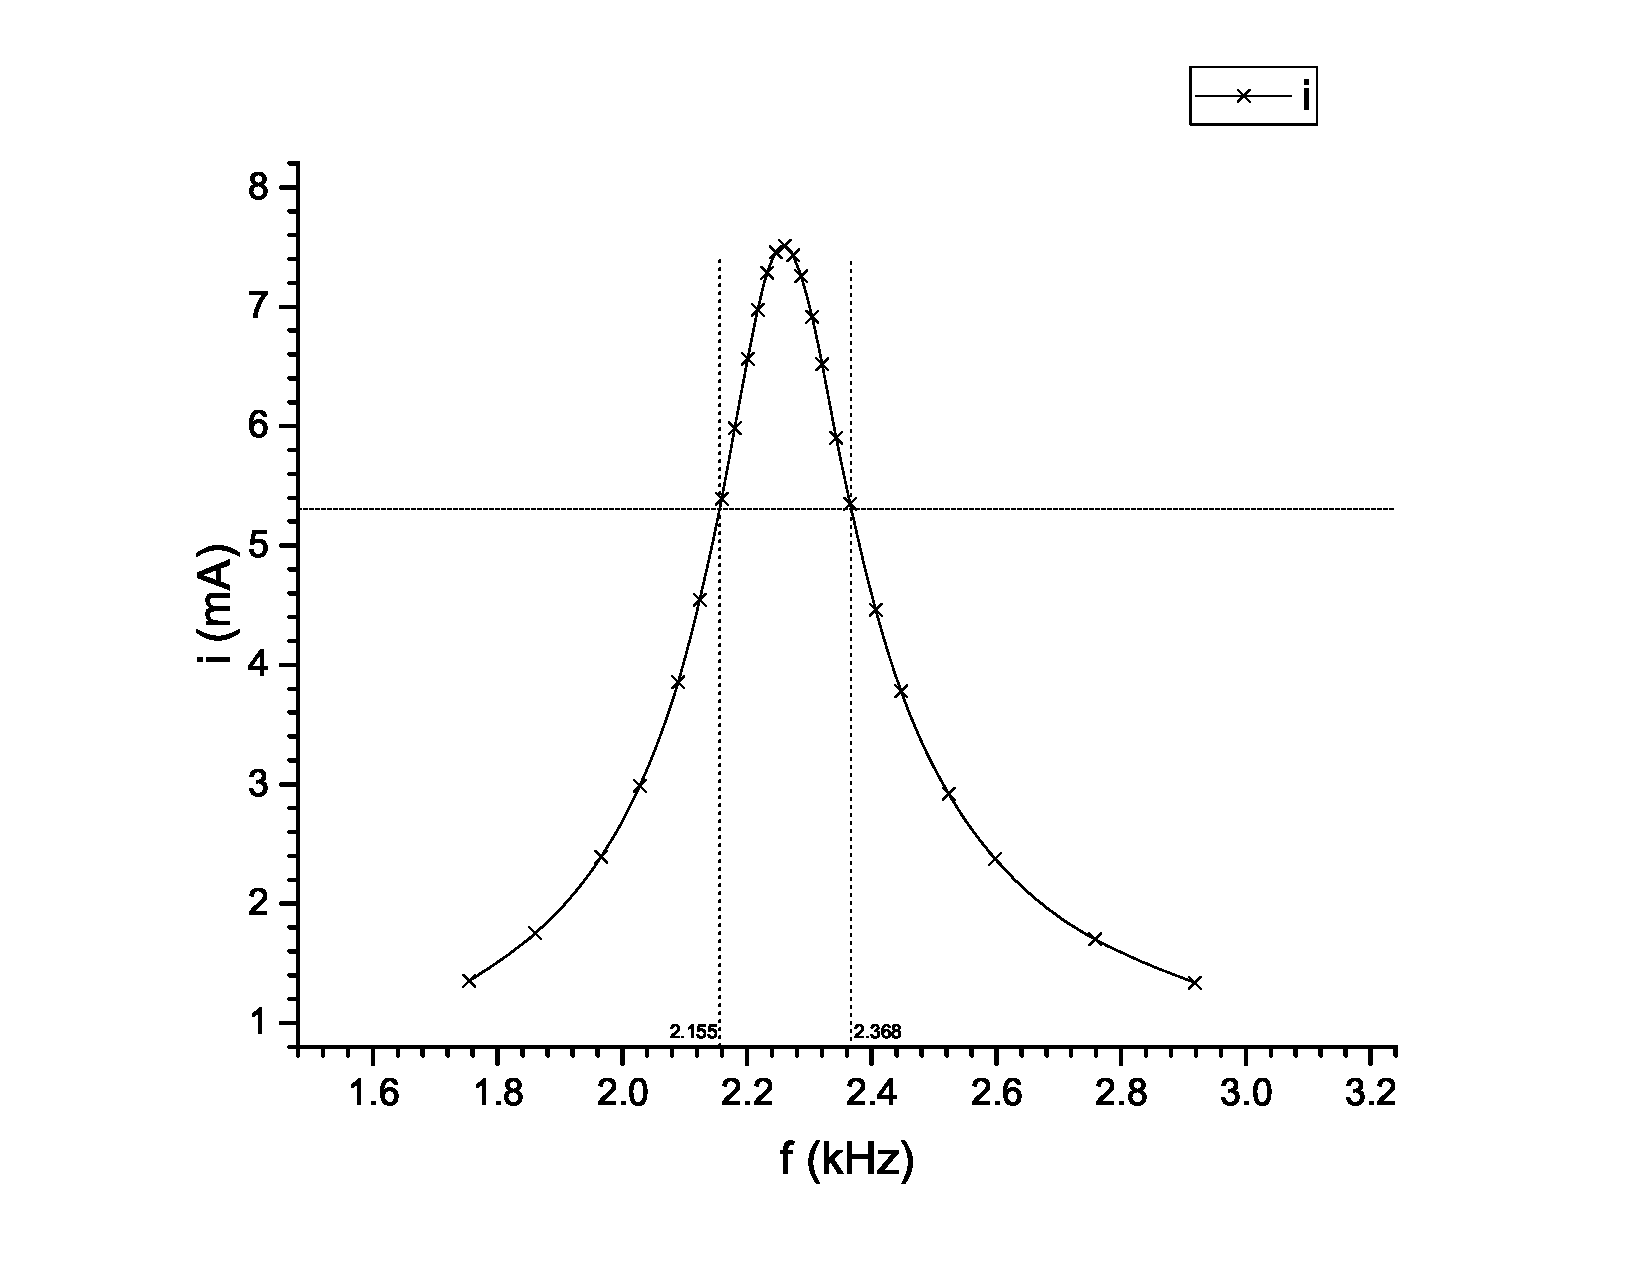
\includegraphics[width=1.0\textwidth]{2}
  \label{fig:digit}
\end{figure}

并借由幅频特性曲线,可读出$\Delta f=0.213 kHz$,故:$$Q_3=\frac{f_0}{\Delta f}=10.61$$

\section{课后思考题}
\subsection{题(1)}
根据电路,有:$$ \left\{
  \begin{aligned}
  |Z| & = & \sqrt{R^2+(\omega L-\frac{1}{\omega C})^2} \\
  \phi & = & \arctan{\frac{\omega L-\frac{1}{\omega C}}{R}} \\
  i & = & \frac {u}{\sqrt{R^2+(\omega L-\frac{1}{\omega C})^2}}
  \end{aligned}
  \right.
  $$

  谐振下,有:
$$ \left\{
\begin{aligned}
f_0 & = & \frac{1}{2\pi\sqrt{LC}} \\
\phi & = & 0 \\
|Z| & = & R \\
i & = & \frac {U}{R}\\
Q & = & \frac{1}{\omega_0RC}
\end{aligned}
\right.
$$

故在已知$L=0.1H,C=0.05\mu F,V_{pp}=3.0V$条件下,进行计算,得:
% Table generated by Excel2LaTeX from sheet 'Sheet1'
\begin{table}[H]
  \centering
  \caption{$R$变化前后对比}
    \begin{tabular}{c|c|c}
    $R=100\Omega$ & $R=500\Omega$ & 变化情况 \\\hline
    $|Z|=100\Omega$ & $|Z|=500\Omega$ & 增大5倍 \\
    $\phi=0$ & $\phi=0$ & 不变 \\
    $i_{pp}=30mA$ & $i_{pp}=6mA$ & 缩小5倍 \\
    $f_0=2.25kHz$ & $f_0=2.25kHz$ & 不变 \\
    $Q=14.1$ & $Q=2.83$ & 缩小5倍 \\
    \end{tabular}%
  \label{tab:addlabel}%
\end{table}%
\subsection{题(2)}
\subsubsection{问(1)}
根据公式$Q=\frac{U_C}{U}$,故可调节$f$使电路谐振。只要此时$f_0$使得$\frac{U_C}{U}$最大时,理论计算有$f=\frac{1}{2\pi\sqrt{LC}}\sqrt{1-\frac{CR_r^2}{L}}$,考虑此时$C$数量级极小,可近似认为此时$f\approx\frac{1}{2\pi\sqrt{LC}}=f_0$,据此判断谐振。计算得$Q$值后,还可以进一步利用公式$Q=\frac{1}{2\pi f_0CR_r}$得$R_r$。由$f_0=\frac{1}{2\pi\sqrt{LC}}$可得$L$。
\subsubsection{问(2)}
\paragraph{1}连接电路;
\paragraph{2}调节$f$并保持$U$不变,当$U_C$出现极大值时,记录$f_0,C,U,U_C$;
\paragraph{3}根据(1)中列出公式完成计算。
\subsubsection{问(3)}
将题中所给数据代入,得:
$$ \left\{
  \begin{aligned}
  Q & = & 100 \\
  R_r & = & 8.04\Omega \\
  L & = & 0.213 mH
  \end{aligned}
  \right.
  $$
  将数据代回,得$\frac{CR_r^2}{L}\sim10^{-7}$,故这个近似是可行的。
  \section{分析与讨论}
  \subsection{各曲线特征及理解}
  \subsubsection{相频特性曲线}
  \paragraph{主要特征}$\phi$随$f$单调上升;当电路处于谐振即$f=f_0$时,$\phi=0$;随着$f$的不断增大,$\phi$趋向于$90^\circ$;随着$f$的不断减小,$\phi$趋向于$-90^\circ$。
  \paragraph{理解}当$f<f_0$时,电路呈电容性,电流相位超前于电压相位,$\phi<0$,随着$f$的不断减小,电路会逐渐趋于(但不能达到)纯电容性,即$\phi$趋于$-90^\circ$;当$f>f_0$时,电路呈电感性,电流相位落后于电压相位,$\phi>0$,随着$f$的不断增大,电路会逐渐趋于(但不能达到)纯电感性,即$\phi$趋于$90^\circ$;
当$f=f_0$时,电路呈纯电阻性,故$\phi=0$。
  \subsubsection{幅频特性曲线}
  \paragraph{主要特征}在$f=f_0$处,存在一极大值。
  \paragraph{理解}考虑$i = \frac {u}{\sqrt{R^2+(\omega L-\frac{1}{\omega C})^2}}$,可以看出,当$f=f_0=\frac{1}{2\pi\sqrt{LC}}$时,分母($|Z|$)有一极小值,故$i$有一极大值。
\subsection{比较三种方法计算所得的$Q$值}
三种方法计算所得$Q$值如下:
$$Q_1\pm\sigma_{Q_1}=10.57\pm0.05$$
$$Q_2\pm\sigma_{Q_2}=10.45\pm0.02$$
$$Q_3=10.61$$

从数值上看,三个$Q$的计算值大致相等,其间的误差,大致可以认为是实验所用的仪器精度所造成。
同时,对于$Q_1$与$Q_2$,由于其采用的测量器具相同,故而精度大致在同一数量级上。

此外,在实际计算中,对于$Q_3$,其计算相对于$Q_1$与$Q_2$较为繁琐。
      \section{收获与感想}
      本次实验,是本学期的最后一个实验,而实验的内容,也是大家所常听闻的电路谐振。

      在进行实验的时候,我通过对$U_C$与$U$的观察,切身感受到了共振现象。而在计算中,也发现三种方法所得的$Q$值大致相等,也感受到理论的精妙。

      从实验中,我从将电路中电流信号,转变为串接电阻的电压信号这一设计,感受到了信号转换的重要性,这一点在过往的实验课程中也一再的强调。

      此外,在本次实验中,我也感受到了自己某些实验能力还有不足,例如电路接线,示波器的使用等,希望在以后的实验课程中,能够提高自己的实验能力。

\end{document} 